\section{Integration into Visualization Tools}

Throughout the lifespan of ECP, the VTK-m team operated in heavy collaboration with other ECP software technology teams.
The scope of the VTK-m portion of the project was to provide the fundamental technology to run scientific visualization algorithms on the GPU processors of the Exascale machines.
Other ECP teams, most notably the ALPINE project, developed tools that would leverage VTK-m while directly addressing application needs.
This arrangement avoided the redundant work of multiple teams developing their own visualization solutions and prevented users from having to use yet another software interface.
In this section we discuss the major visualization tools we integrated VTK-m with.

\ken{
  Each subsection should be roughly 1/2 page plus have an image demonstrating the tool with VTK-m that is about 1/3 page.
  (3 + 1/3 page total.)
  The subsection should start with a description of the tool.
  (Exception: the last subsection starts with a description of the lengthy process from committing code in VTK-m to it being available in a tool.)
  The following paragraphs describe how VTK-m is integrated at a high level.
  Avoid details like classnames.
}

\subsection{ParaView}

\assign{Sujin}
The VTK-m library provides high performance implementations of several visualization algorithms for highly parallel processors. However, features such as file IO, rendering, pipeline management, etc, which are essential parts of a full featured visualization toolkit, are beyond the scope of VTK-m. On the other hand, ParaView is a mature visualization software that has robust implementation of these features. Therefore, we wanted to integrate VTK-m into ParaView, such that ParaView can use VTK-m filters to accelerate its operations, when a VTK-m implementation and highly parallel hardware is available.

We wanted to make the use of VTK-m accelerated filters as transparent as possible. Therefore, we have chosen to integrate VTK-m using VTK and ParaView’s factory-instantiation feature. Filter in ParaView are instantiated via a factory method. There can be multiple implementations available for a filter and the factory method chooses an appropriate implementation at run-time based on some criteria. With this method we can override the default ParaView filters with VTK-m based filters. Currently, VTK-m accelerated overrides are available for some commonly used filters such as Contour, Threshold, Gradient, etc. Adding overrides for more filters is a fairly straightforward process as discussed in the following paragraphs.

To override a ParaView filter, we first need to implement a VTK-m wrapper filter in VTK, that provides the interface of the base VTK/ParaView filter and uses VTK-m filters and routines for its operation. The following steps give a high-level overview of how a VTK-m wrapper filter is implemented in VTK/ParaView.
\begin{itemize}
    \item Check the filter parameters and only proceed with VTK-m processing for configurations supported by the VTK–m filter implementation.
    \item Convert the input VTK datasets to VTK-m datasets. 
    \item Execute the VTK-m filter on the data.
    \item Convert the output of the VTK-m filter back to VTK datasets
    \item If at any point during the above steps, there is an error, fall-back to the default VTK implementation. Errors in VTK-m are typically signaled via C++ exceptions.
\end{itemize}

For the dataset conversion from VTK to VTK-m and back, we have implemented several helper routines. These are zero-copy operations for most cases as only the ownership of the pointers to the underlying resources are transferred wherever possible. Even copy from host to device and device to host are minimized with the use of a VTK-m dataset wrapper in VTK called \texttt{vtkmDataSet}, that implements the interface of \texttt{vtkDataSet} and only copies the data when required. Another commonly used ParaView functionality, of computing the range of the various fields of a dataset, has also been accelerated using VTK-m to speed up the computation and to avoid memory transfer from device to host.

The wrapper filter needs to be registered with the factory for the factory instantiation to work. This is done at the build configure time using the CMake function:
\texttt{\_vtkm\_add\_override("vtkBaseFilter" "vtkmAcceleratedFilter")} Thne, the accelerated filters need to be enabled using the CMake option \texttt{VTK\_ENABLE\_VTKM\_OVERRIDES}. They can also be turned on or off during run time through ParaView settings as shown in Figure~\ref{fig:paraview_settings}.

\begin{figure}[htb]
  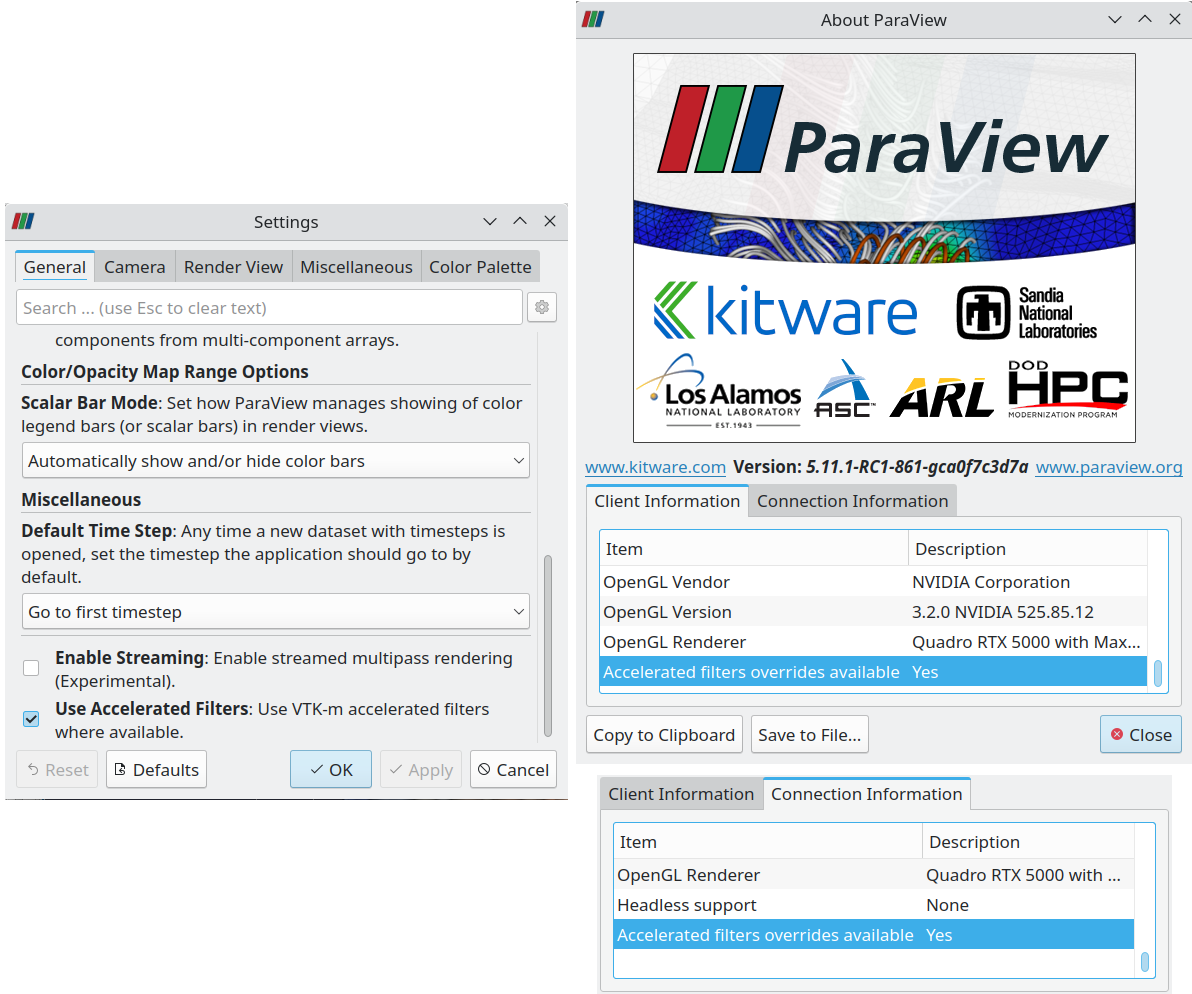
\includegraphics[width=\linewidth]{figures/pv-override-settings.png}
  \caption{Left: ParaView setting \texttt{Use Accelerated Filters} can be used to turn on or off accelrated filters at run-time. This setting is shown irrespective of whether ParaView was built with the override support or not. Right: The availability of the accelerated filters can be found under \texttt{About ParaView/Client Information} for clients and \texttt{About ParaView/Connection Information} for servers.}
  \label{fig:paraview_settings}
\end{figure}


\subsection{VisIt}

\assign{Eric}
VisIt is a scientific visualization and analysis tool that operates on mesh-based field data. Its functionality is grouped into four major categories: Plots, Operators, Expressions and Queries. All four of these capabilities are built on a filter infrastructure that operates on mesh-based fields. Plots are somewhat special in that they consist of a rendering capability that may include some built-in filter operations. The VTK-m integration to date has consisted of modifying the filter infrastructure to use VTK-m filters where there exists comparable VTK-m functionality. There has not yet been an effort to utilize VTK-m’s rendering capabilities.

Previously, VisIt’s filters used VTK filters and VTK data sets. The filters were enhanced to support using both VTK and VTK-m. When VTK-m is enabled in VisIt and the filter supports VTK-m, the filter will use VTK-m. The internal data set representation was also modified to support providing either a VTK data set or a VTK-m data set. When the filter wants to use VTK, it will request the data as a VTK data set and convert the data set to a VTK data set if it is stored as a VTK-m data set. Conversely, when the filter wants to use VTK-m, it will request the data as a VTK-m data set and convert it if necessary. When doing the conversions, it will use zero-copy conversions wherever possible.

\begin{figure}[htb]
  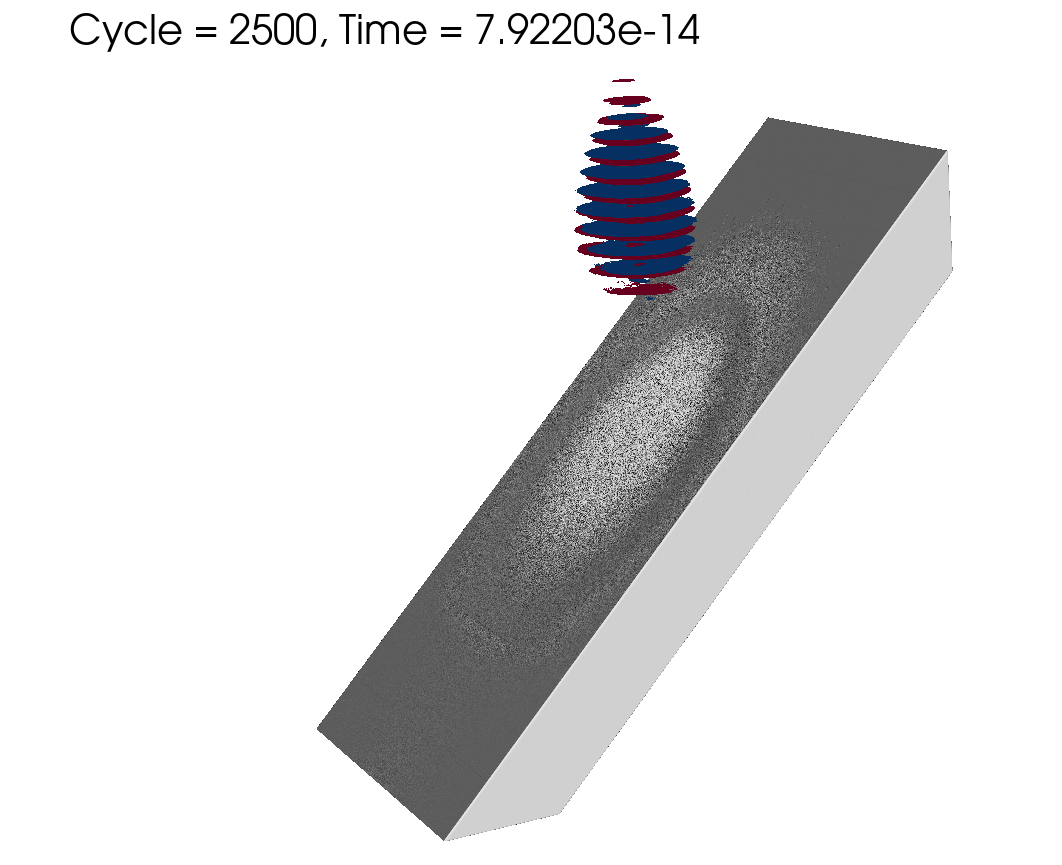
\includegraphics[width=\linewidth]{figures/visit_warpx_frontier.png}
  \caption{Visualization from a 70 billion cell WarpX Gordon Bell simulation visualized with 2048 GPUs on Frontier.}
  \label{fig:visit_warpx_frontier}
\end{figure}

Figure~\ref{fig:visit_warpx_frontier} is an image generated by VisIt running on Frontier using 2048 GPUs on 256 nodes. The surfaces were generated using the VTK-m Contour filter and were rendered in parallel using Mesa 3D. VTK-m is using the Kokkos backend for AMD GPUs.

\subsection{Ascent}
\assign{Nicole}
Ascent is a lightweight in situ visualization and analysis library designed for multi-physics HPC simulations. As an in situ library, as opposed to a post-hoc visualization tool, Ascent shares execution resources with the simulation and can process the data as it is generated, reducing I/O costs, though it has to pause the simulation to do so. To minimize the encumbrance on the simulation and execution resources, Ascent’s lightweight design ensures a small memory requirement. It is written using efficient distributed-memory and many-core libraries to guarantee performance and scalability on current and next-generation HPC platforms. Ascent has three main use cases: making pictures, transforming data, and capturing data. And aims to be easy-to-use with only five API calls supported in C, C++, Python, and Fortran, while also providing an infrastructure to integrate custom analysis.

VTK-m, while optional, is a main dependency for Ascent, as it is currently the only option for rendering low-order mesh data offered in Ascent, and provides filters for transforming and/or analyzing the simulation data e.g. Slice, Histogram, Isosurface. Ascent also takes advantage of VTK-m’s zero-copy capabilities as well as its ability to pass device-pointers, allowing the simulation data to remain on the device and be passed directly to Ascent, and then VTK-m, without having to be transferred to host memory. VTK-m has been integrated into Ascent via a (previously external) library called VTK-h (the “h” meaning “hybrid”), that combines VTK-m’s shared-memory performant filters with MPI’s efficient distributed-memory coordination. 

Figure~\ref{fig:warpx_lwfa} is an in situ rendering of the WarpX simulation (see section \textit{Laser Wakefield Acceleration}), generated by Ascent, executing on OLCF's exascale supercomputer Frontier.
The simulation was executed in two resolutions: 578.8 million cell across 552 GPUs on 69 nodes and 4.63 billion cells across 4,416 GPUs on 552 nodes (inset).
Ascent used VTK-m filters to upscale the data along multiple axis, generate isosurfaces, and clip several fields, before using VTK-m's raytracer and volume renderer to generate the final image.
To guarantee performance, VTK-m uses the Kokkos backend for AMD GPUs. 

\begin{figure}[htb]
  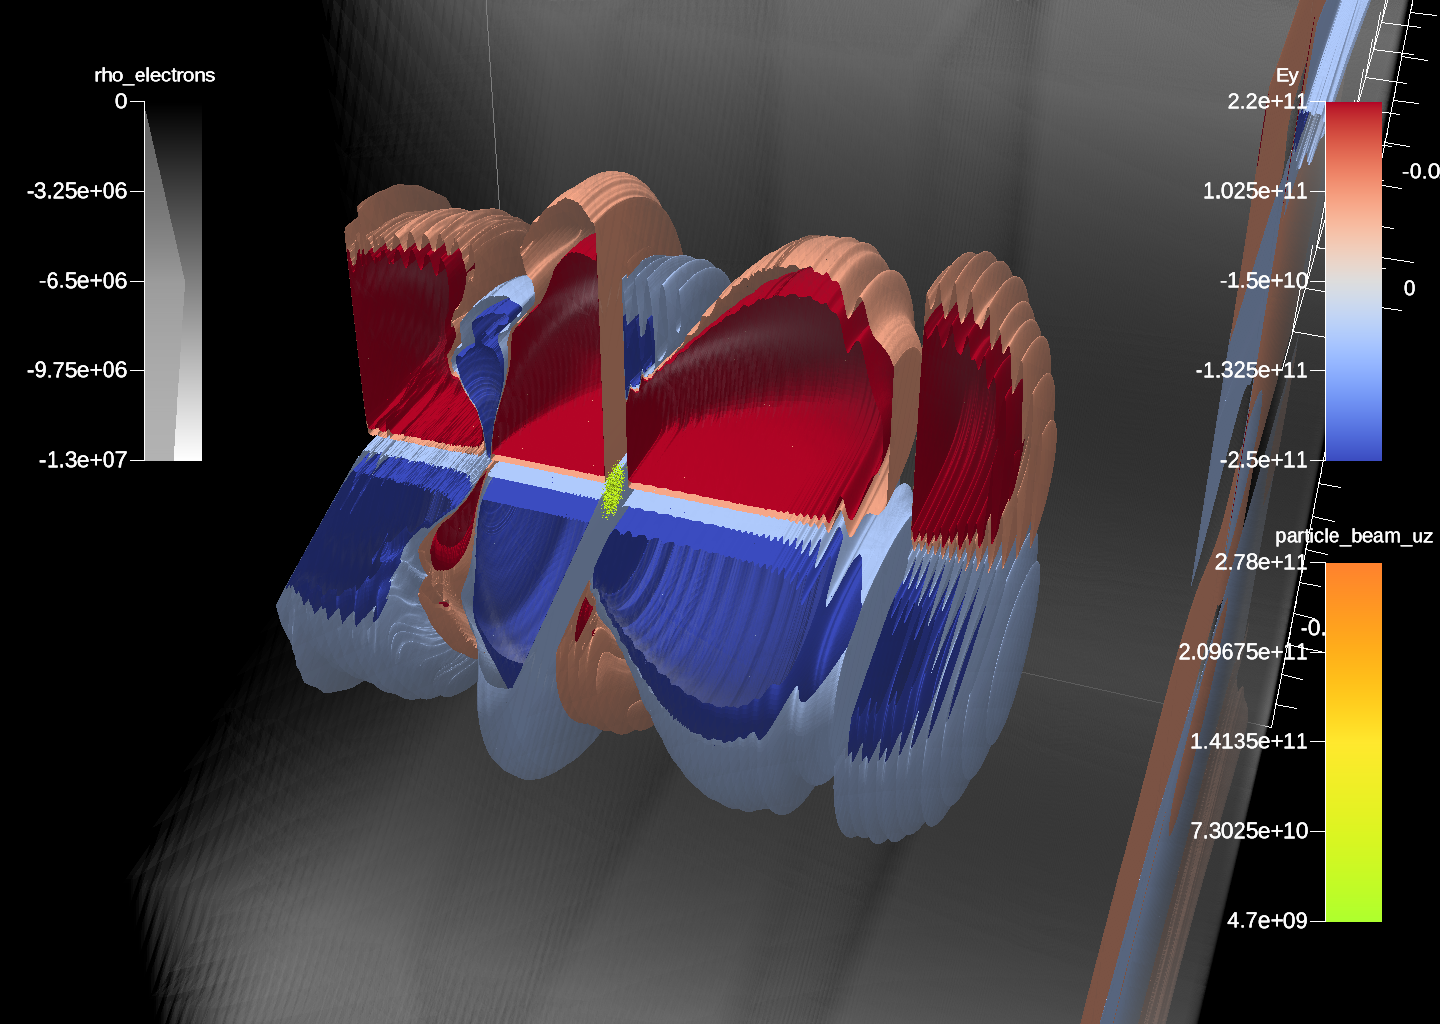
\includegraphics[width=\linewidth]{figures/warpx_stages_lwfa.png}
  \caption{WarpX in situ visualization of laser-wakefield accelerator on 552 and 4,416 Frontier GPUs using Ascent and VTK-m.
  The inset shows an early simulation time step at high resolution.}
  \label{fig:warpx_lwfa}
\end{figure}

\subsection{Alternate Delivery Mechanisms}

\assign{Tushar}
Integrating VTK-m filter into visualization software, e.g., ParaView, and VisIt, can be a lengthy process. For example, making a VTK-m filter available in ParaView requires going through multiple steps, including implemention of a VTK filter that wraps the VTK-m filter, continuous integration for VTK wrapper, and similar steps in ParaView. Such time-consuming software integration process can hinder the accessibility of VTK-m filters inside visualization tools, thus rendering VTK-m filters less effective in enhancing the pace of scientific discovery. 

Our ultimate goal is to make VTK-m filters practical for real use and to put tools in the hands of end users in a timely manner. One of the benefits that VTK-m offers is the easy exportation of VTK-m filters as plugins, which circumvents the tedious software integration process and makes VTK-m filters usable in ParaView and VisIt. For the plugin approach, the VTK-m filter still needs to be wrapped inside a VTK filter, but the time needed for the software integration and testing in VTK and ParaView can be bypassed.       

\begin{figure}[htb]
  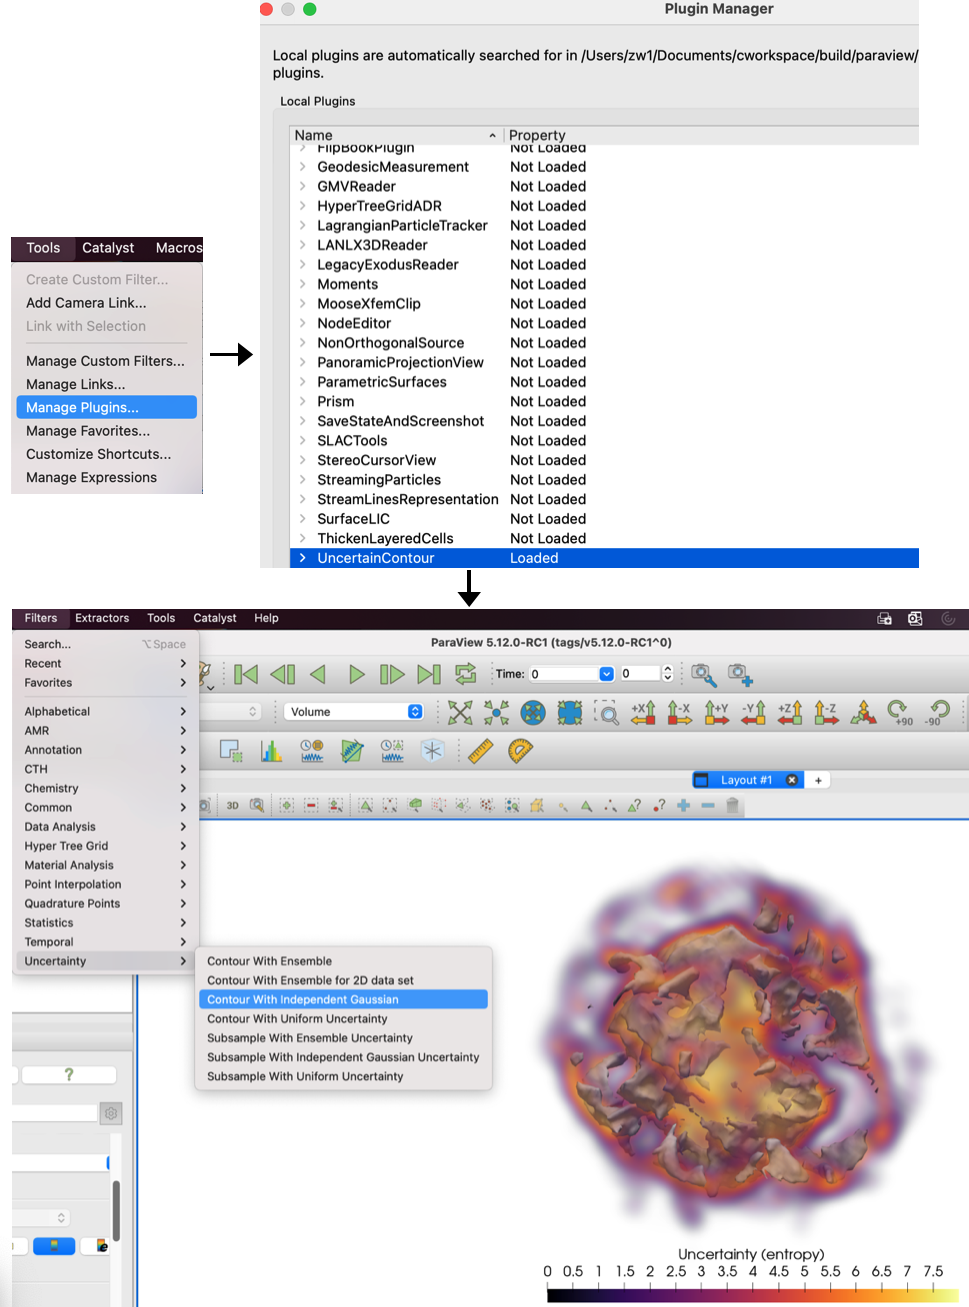
\includegraphics[width=\linewidth]{figures/isosurfaceUncertaintyPlugin.png}
  \caption{Integration of the VTK-m isosurface uncertainty filter into ParaView using the plugin approach for visualization of large-scale supernova simulations~\cite{Sandoval2021}.}
  \label{fig:uncertainty-plugin}
\end{figure}

Figure~\ref{fig:uncertainty-plugin} illustrates the VTK-m isosurface uncertainty filter made available in ParaView using the plugin method. The isosurface uncertainty filter~\cite{Wang2023} is one of the major successes of the VTK-m library, as it is the first production-level uncertainty visualization filter deployed for efficient large-data analysis. The filter enables interactive exploration of uncertainty in marching cubes topology cases~\cite{Athawale21} and overcomes difficulties related to the slowness of uncertainty computations. \tushar{Should we add here a link to the uncertainty filter in the master branch and add Nrushad as author?}. Using the plugin method depicted in Figure~\ref{fig:uncertainty-plugin}, VTK-m filters can be easily coupled with existing filters in ParaView for faster and better data understanding.

\ken{
  Talk about how you can deliver new functionality to these tools outside of the pipeline of implement in VTK-m $\rightarrow$ VTK $\rightarrow$ Tool.
  Use uncertainty plugin as an example of doing this.
}
